\documentclass[tikz,border=0pt]{standalone}
\usepackage[american]{circuitikz}
\usetikzlibrary{arrows.meta,calc,positioning,decorations.pathmorphing,patterns}
\definecolor{zyloTeal}{HTML}{174A5B}
\definecolor{zyloTealTwo}{HTML}{246B7A}
\definecolor{zyloInk}{HTML}{1F2933}
\definecolor{zyloSoft}{HTML}{EAF4F4}
\definecolor{zyloPaper}{HTML}{F8FAFB}
\definecolor{zyloLine}{HTML}{44606B}
\definecolor{zyloOrange}{HTML}{D97706}
\begin{document}
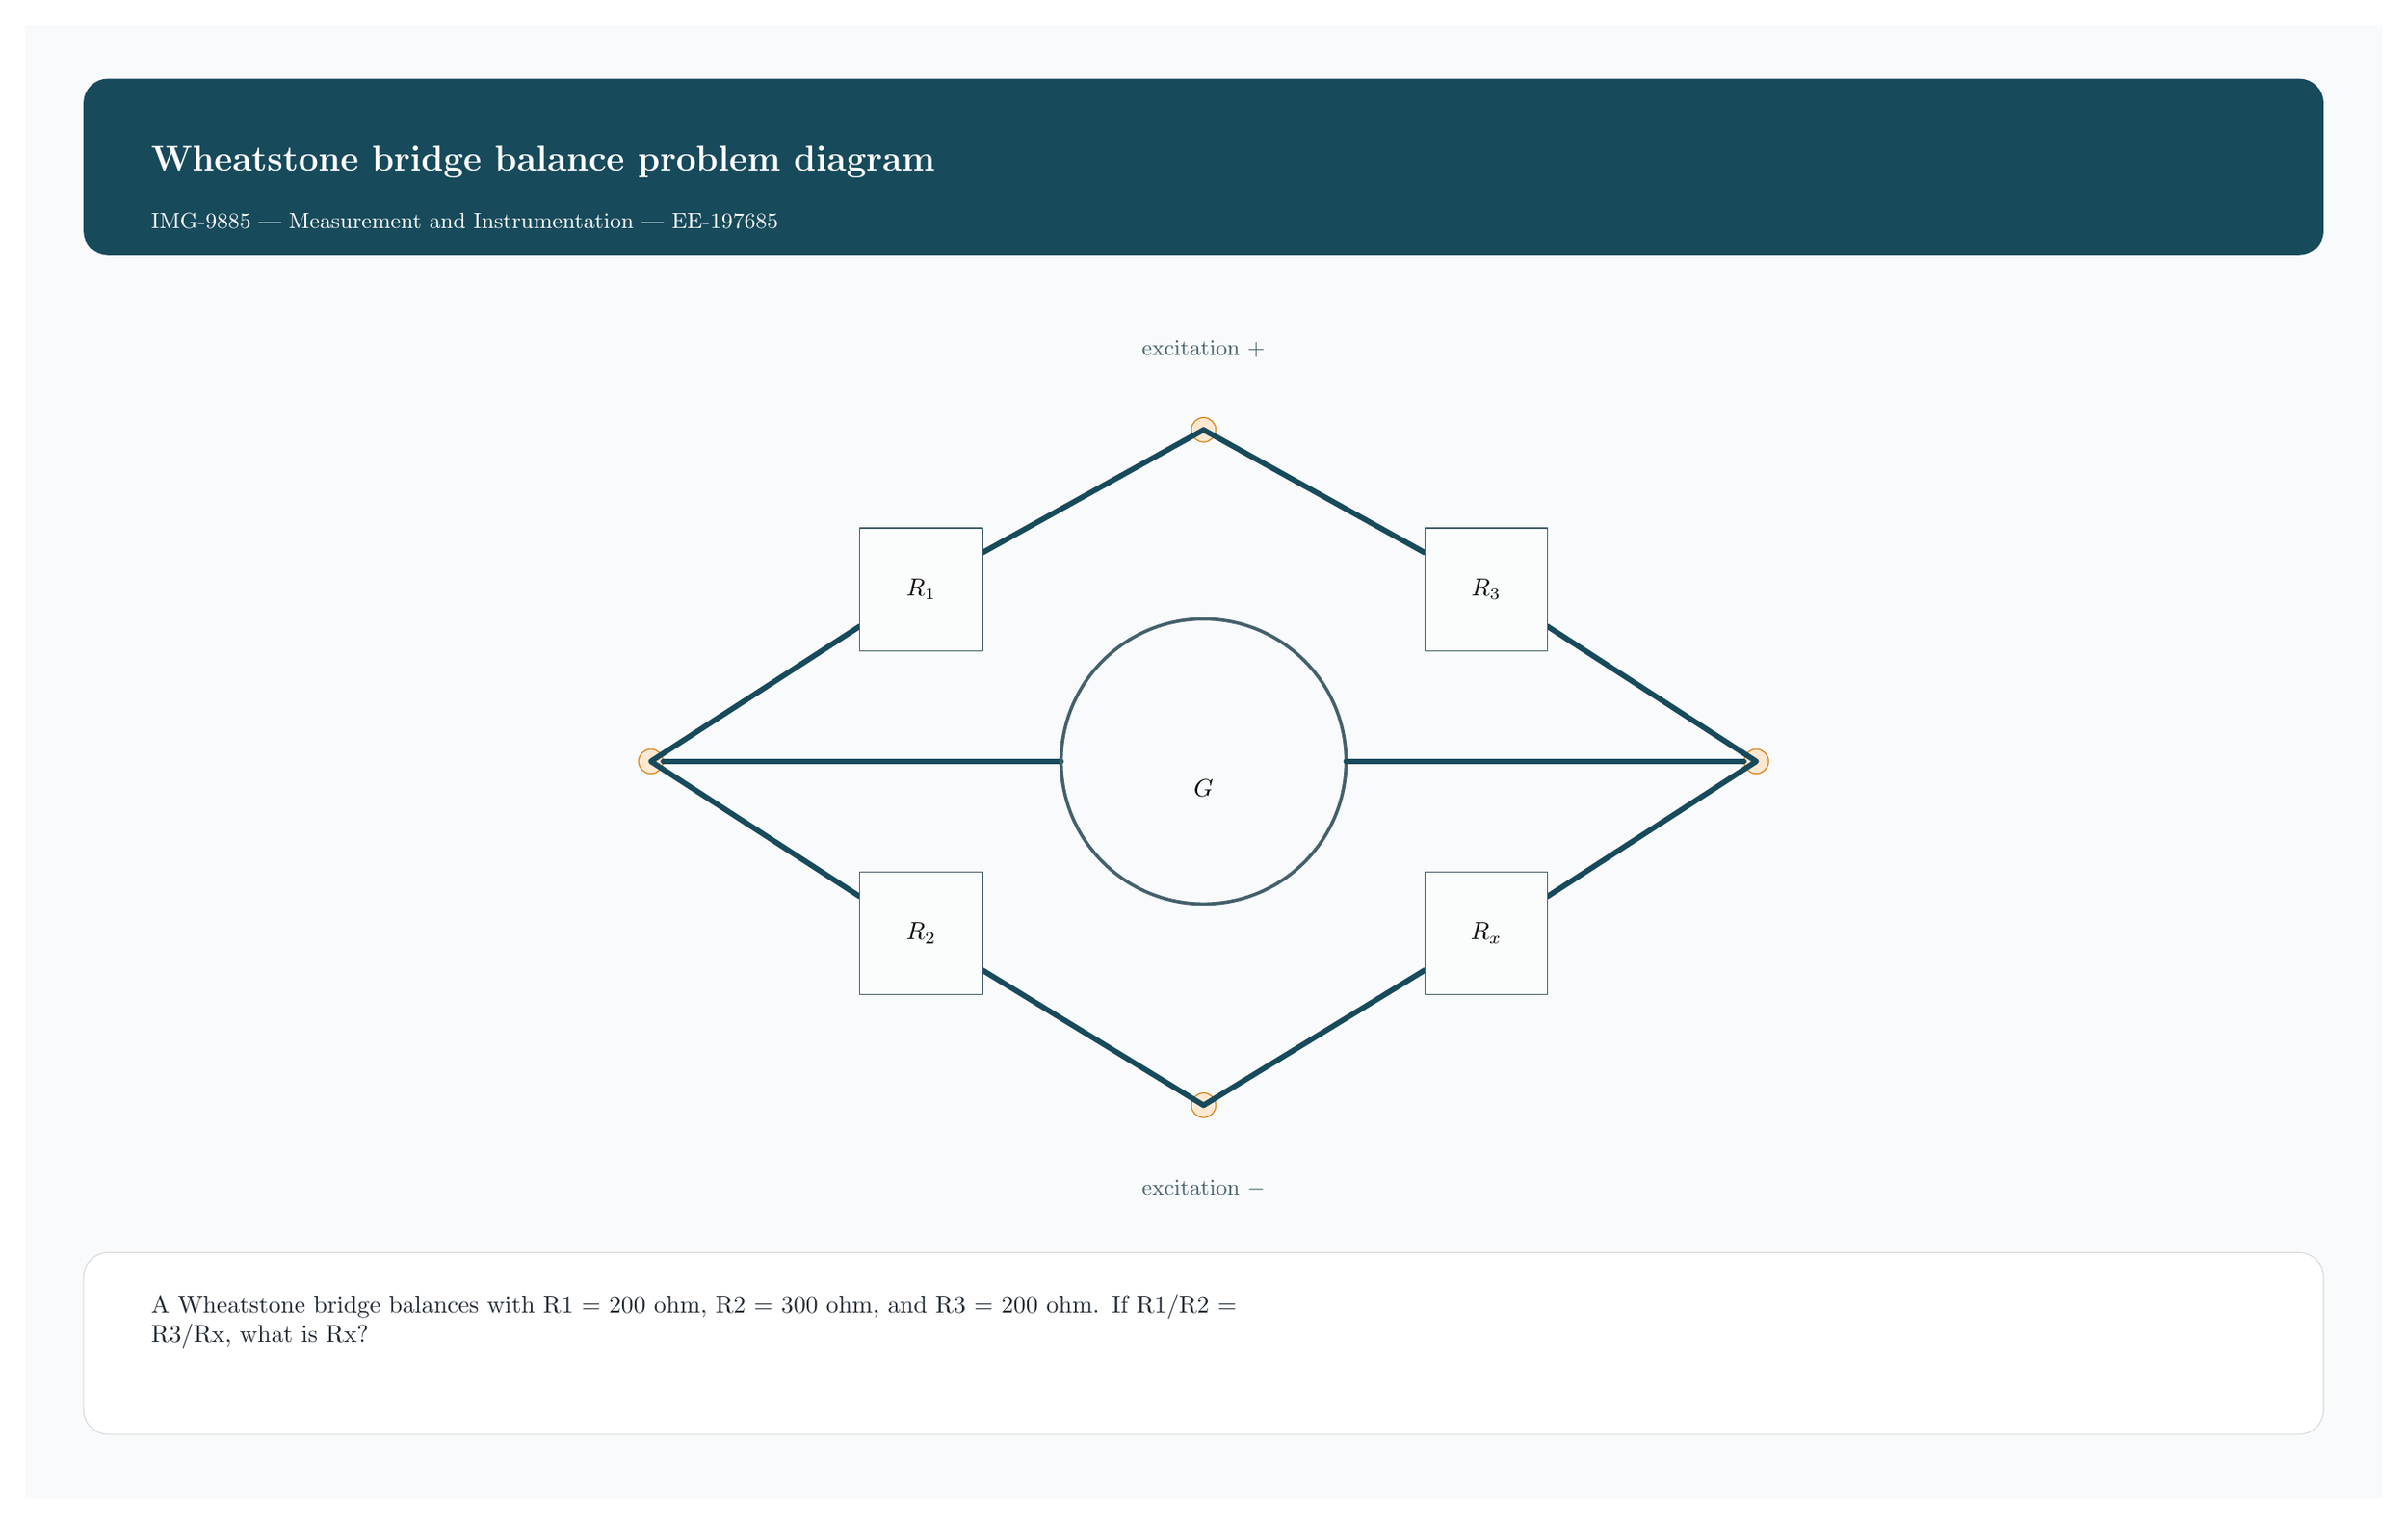
\begin{tikzpicture}[x=1pt,y=-1pt,>=Latex,line cap=round,line join=round]
\path[fill=zyloPaper] (0,0) rectangle (960,600);
\path[fill=zyloTeal,rounded corners=10pt] (24,22) rectangle (936,94);
\node[anchor=west,text=white,font=\bfseries\Large] at (48,56) {Wheatstone bridge balance problem diagram};
\node[anchor=west,text=white!82,font=\small] at (48,80) {IMG-9885 | Measurement and Instrumentation | EE-197685};
\tikzset{wire/.style={draw=zyloTeal,line width=2.2pt},thinwire/.style={draw=zyloLine,line width=1.35pt},accent/.style={draw=zyloOrange,line width=2.2pt},box/.style={draw=zyloTealTwo,fill=zyloSoft,line width=1.5pt,rounded corners=8pt}}
\filldraw[draw=zyloOrange,fill=orange!18] (480,165) circle (5); \filldraw[draw=zyloOrange,fill=orange!18] (480,440) circle (5);
\filldraw[draw=zyloOrange,fill=orange!18] (255,300) circle (5); \filldraw[draw=zyloOrange,fill=orange!18] (705,300) circle (5);
\draw[wire] (480,165) -- (390,215); \draw[wire] (340,245) -- (255,300) -- (340,355); \draw[wire] (390,385) -- (480,440);
\draw[wire] (480,165) -- (570,215); \draw[wire] (620,245) -- (705,300) -- (620,355); \draw[wire] (570,385) -- (480,440);
\node[draw=zyloLine,fill=white!80!zyloSoft,minimum width=50pt,minimum height=50pt] at (365,230) {$R_1$};
\node[draw=zyloLine,fill=white!80!zyloSoft,minimum width=50pt,minimum height=50pt] at (365,370) {$R_2$};
\node[draw=zyloLine,fill=white!80!zyloSoft,minimum width=50pt,minimum height=50pt] at (595,230) {$R_3$};
\node[draw=zyloLine,fill=white!80!zyloSoft,minimum width=50pt,minimum height=50pt] at (595,370) {$R_x$};
\draw[wire] (260,300) -- (422,300); \draw[thinwire] (480,300) circle (58); \node at (480,311) {$G$}; \draw[wire] (538,300) -- (700,300);
\node[font=\small,text=zyloLine] at (480,132) {excitation $+$}; \node[font=\small,text=zyloLine] at (480,474) {excitation $-$};
\path[draw=black!15,fill=white,rounded corners=10pt] (24,500) rectangle (936,574);
\node[anchor=west,text width=860pt,align=left,text=zyloInk,font=\normalsize] at (48,528) {A Wheatstone bridge balances with R1 = 200 ohm, R2 = 300 ohm, and R3 = 200 ohm. If R1/R2 =\\R3/Rx, what is Rx?};
\end{tikzpicture}
\end{document}
